% Type de rupture
\begin{frame}{Différents types de rupture}{Définition}
\begin{block}{Définition}

Il existe plusieurs types de rupture, les différents types de rupture influencent le choix de la taille de fenêtre, la précision du résultat, etc. 

\begin{itemize}
    \item Changement d'image ;
    \item Fondu d'image ;
    \item etc.
\end{itemize}

\end{block}

\end{frame}

% Exemple de rupture
\begin{frame}{Rupture}{Exemples}

\begin{figure}
   \begin{minipage}[c]{.46\linewidth}
	  \centering
      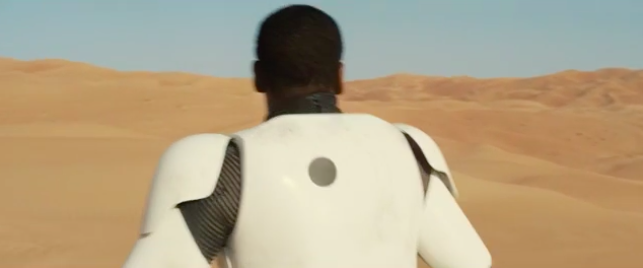
\includegraphics[scale=0.2]{images/rupture1-1.png}
      \caption{Avant}
   \end{minipage} \hfill
   \begin{minipage}[c]{.46\linewidth}
      \centering
      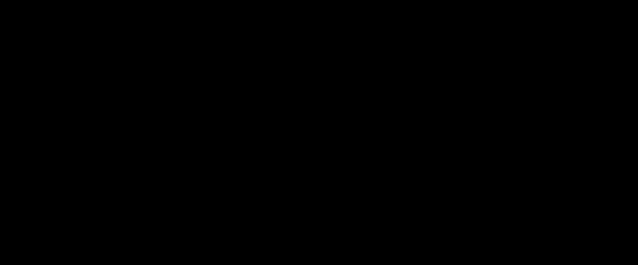
\includegraphics[scale=0.2]{images/rupture1-2.png}
      \caption{Après}
   \end{minipage}
\end{figure}

\begin{figure}
   \begin{minipage}[c]{.46\linewidth}
	  \centering
      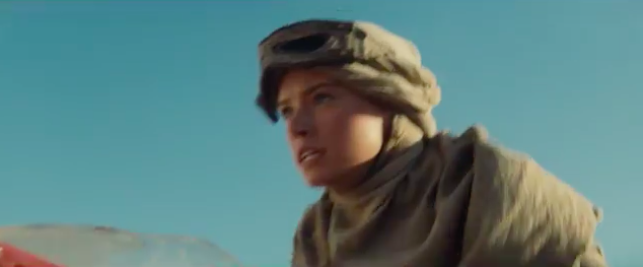
\includegraphics[scale=0.2]{images/rupture2-1.png}
      \caption{Avant}
   \end{minipage} \hfill
   \begin{minipage}[c]{.46\linewidth}
      \centering
      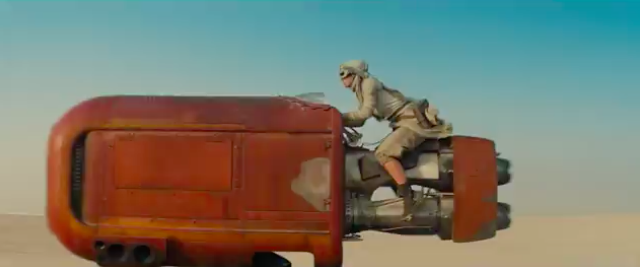
\includegraphics[scale=0.2]{images/rupture2-2.png}
      \caption{Après}
   \end{minipage}
\end{figure}

\end{frame}

% RGB
\begin{frame}{RGB}{Définition}
\begin{block}{Définition}
La matrice RGB contient les informations des trois couleurs des frames d'une vidéo. L'information de chaque couleur est représenté par 256 niveaux.

La structure de cette matrice est en deux dimensions:

\begin{itemize}
	\item Première dimension: 
		\begin{itemize}
			\item Taille: (3 couleurs) * (256 niveau);
			\item Nombre d'occurence de chaque niveau de couleur.
		\end{itemize}
	\item Seconde dimension: Différents frames.
\end{itemize}

\end{block}

\end{frame}

% Conclusion
\begin{frame}{RGB}{Conclusion}

\begin{block}{Avantages :}

\begin{itemize}
    \item Simple à mettre en oeuvre ;
    \item Relativement robuste à l'apparition de nouveaux objets sur une scène.
\end{itemize}

\end{block}

\begin{block}{Inconvénients :}

\begin{itemize}
    \item Peu robuste aux transition avec un effet de fondu .
\end{itemize}

\end{block}

\end{frame}

% YCbCr
\begin{frame}{YCbCr}{Définition}
\begin{block}{Définition}
YCbCr est une manière de représenter l'espace colorimétrique en vidéo. Y représente la densité de la lumière. Cb et Cr sont les deux informations de chrominance. Cb=(Y-bleu), Cr=(Y-rouge).

\begin{itemize}
	\item Première dimension: 
		\begin{itemize}
			\item Taille: (3 couleurs) * (256 niveau);
			\item Nombre d'occurence de chaque niveau de couleur.
		\end{itemize}
	\item Seconde dimension: Différents frames.
\end{itemize}

\end{block}

\end{frame}

% Relation YCbCr et RGB
\begin{frame}{YCbCr}{Conversion RGB YCbCr}

\begin{exampleblock}{Conversion}
\[
 \left \{
 \begin{array}{c @{=} l}
	Y & 0.299 * R + 0.587 * G + 0.114 * B \\
	Cb & -0.1687 * R - 0.3313 * G + 0.5 * B + 128 \\
	Cr & 0.5 * R - 0.4187 * G - 0.0813 * B + 128 \\
 \end{array}
 \right.
\]

\[
 \left \{
 \begin{array}{c @{=} l}
	R & Y + 1.402 * (Cr - 128) \\
	G & Y - 0.34414 * (Cb - 128) - 0.71414 * (Cr - 128) \\
	B & Y + 1.772 * (Cb - 128) \\
 \end{array}
 \right.
\]
\end{exampleblock}

\end{frame}

% Exemple
\begin{frame}{YCbCr}{Exemples}

\begin{figure}
      \centering
      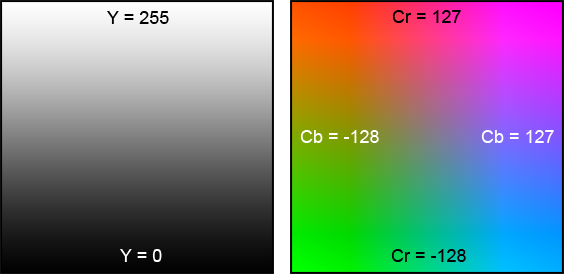
\includegraphics[scale=0.5]{images/YCbCr.png}
      \caption{YCbCr}
\end{figure}

\end{frame}

% Conclusion
\begin{frame}{YCbCr}{Conclusion}

\begin{block}{Avantages :}

\begin{itemize}
    \item Simple à mettre en oeuvre, plus efficace que codage RGB ;
    \item Relativement robuste à l'apparition ou la disparition d'un objet sur une scène.
\end{itemize}

\end{block}

\begin{block}{Inconvénients :}

\begin{itemize}
    \item Peu robuste aux transitions avec un effet de fondu .
\end{itemize}

\end{block}

\end{frame}

